

\section{Bridging languages: How do you say anchor in Chinese?}
\label{sec:mtanchor}


\begin{figure}
  \centering
  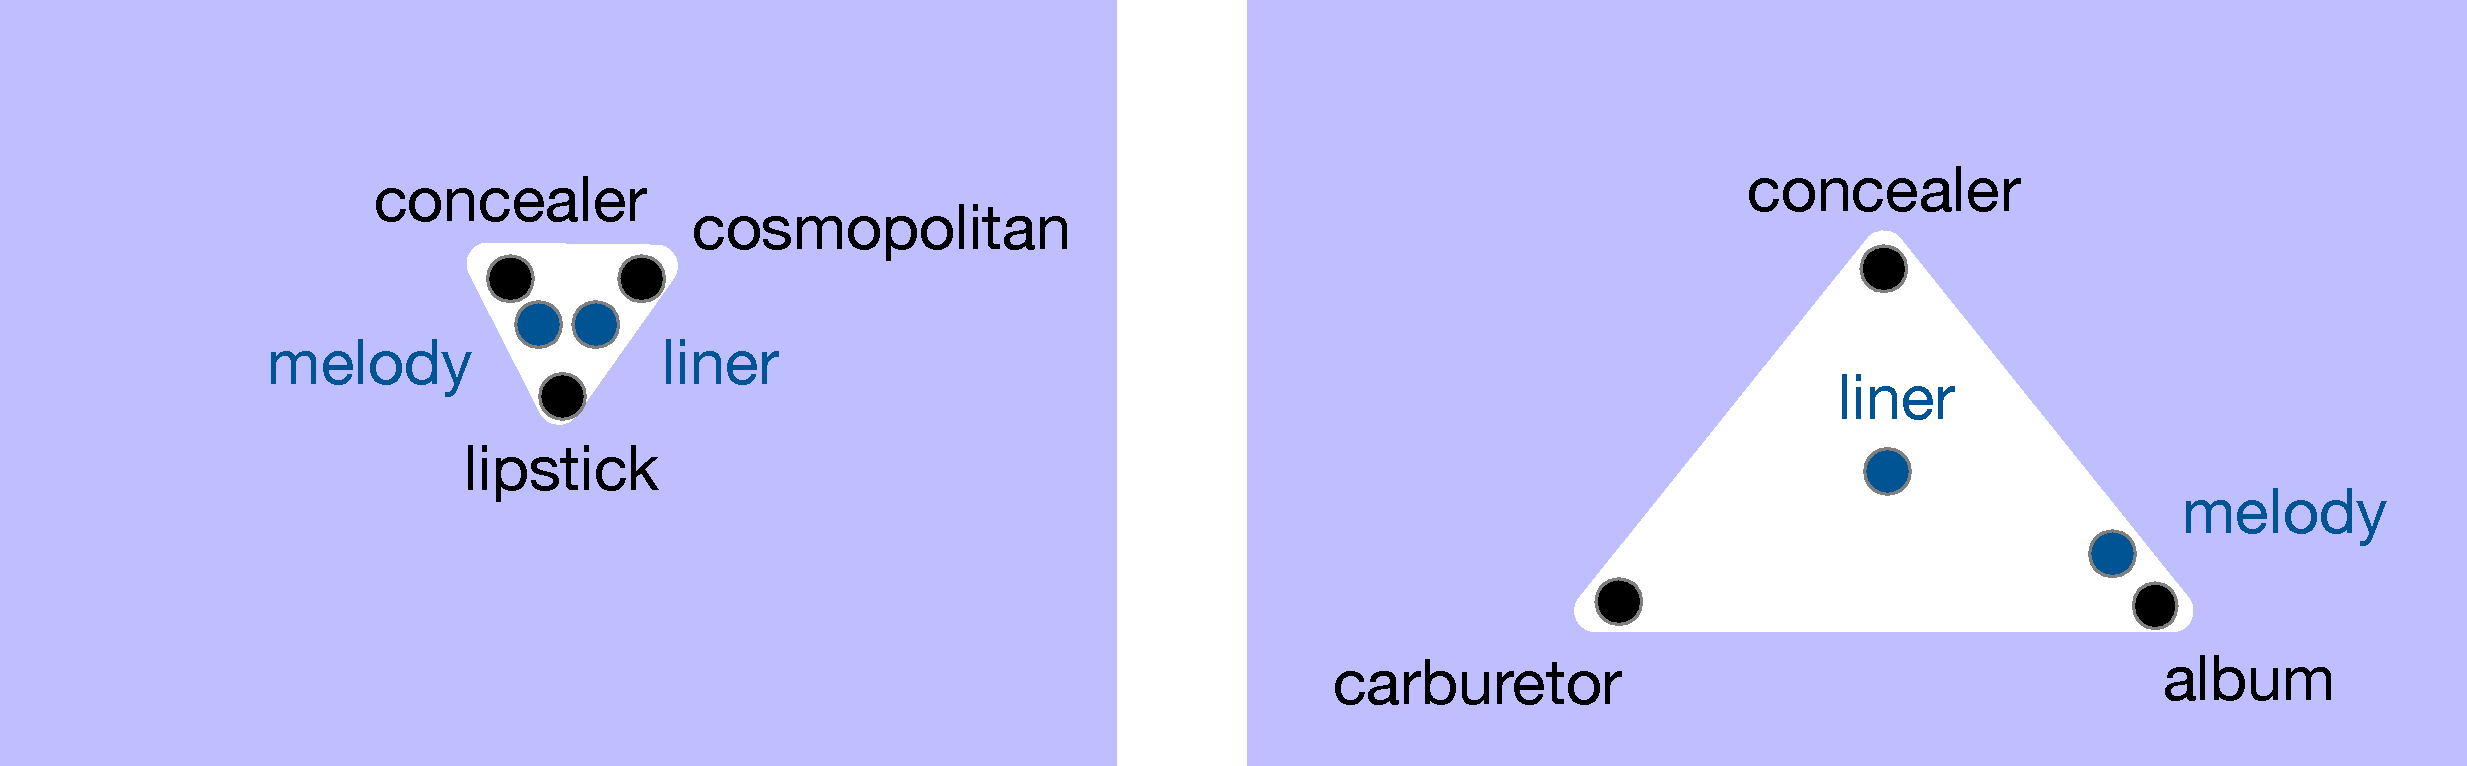
\includegraphics[width=\textwidth]{span.pdf}
  \caption{Visualizing the importance of choice in anchor words for approximating conditional distributions.  The chosen anchor words are the black dots and their span is the white triangle.  On the left, the span of anchor words is small, so the words ``melody'' and ``liner'' are too close together.  On the right, the span of anchor words is large, so the conditional distributions of words ``melody'' and ``liner'' are approximated more accurately.}
  \label{fig:span}
\end{figure}

Anchor-based topic models are well-defined for individual languages, but a
multilingual model requires topics that are thematically connected across languages.  Discovering two separate sets of anchor words does not suffice.
In this section, we propose multilingual anchoring as an algorithm to cross-lingually link topics and their corresponding anchor words.


First, we can connect anchor words across languages as \emph{anchor links}.  For example,
``anchor'' may be linked to ``\zh{錨}{(m\'ao)}'' in Chinese under a
\underline{nautical} context.  After anchor words are linked, all words in the same topic across languages will be form a coherent multilingual topic. A straightforward way to link words across
languages is through a \emph{dictionary}, much as a human would.
Just as possessing a Chinese dictionary does not enable someone to speak Chinese, a dictionary does not magically create multilingual topics.  To construct an overall coherent model, anchor links should be carefully selected.

We define these links in more detail.  A language~$\mathcal{L}$ is a
set of word types~$w$.   A bilingual dictionary~$\mathcal{B}$ is a subset of the Cartesian product~$\mathcal{L}^{(1)} \times \mathcal{L}^{(2)}~$, 
where~$\mathcal{L}^{(1)}, \mathcal{L}^{(2)}$ are two different languages.  An element~$(w^{(1)}, w^{(2)})$
of~$\mathcal{B}$ represents a dictionary entry where words~$w^{(1)} \in \mathcal{L}^{(1)}$
and~$w^{(2)} \in \mathcal{L}^{(2)}$ are translations of each other. While~$\mathcal{B}$ is a
binary relation, it is not necessarily a function.  Other multilingual
topic models require that the dictionary is a one-to-one
correspondence~\cite{jagarlamudi-2010,
  boyd-graber-2009,gutierrez-2016}.  We relax this restriction on
$\mathcal{B}$ to extract as much information from the
dictionary as possible.

We could select anchor words~$s_1,...,s_K$ \emph{independently}
for each language by considering all
words~$w^{(1)} \in \mathcal{L}^{(1)}$ and~$w^{(2)} \in \mathcal{L}^{(2)}$ as
possible candidates for anchors (e.g., independent runs of anchor
algorithm).  Instead, we want to \emph{jointly} choose anchor words for
both languages.  First, we use dictionary entries to create \emph{links} between words.  Then, we choose anchor words~$s_k^{(1)}$ for Language~1 and
$s_k^{(2)}$ for Language~2 such that
$s_k^{(1)}$ and~$s_k^{(2)}$ are linked.  Through this process, we obtain a set of
$K$ anchor words for each language and can obtain topics using
RecoverL2~\cite{arora-2013}. 

\begin{figure}
  \centering
  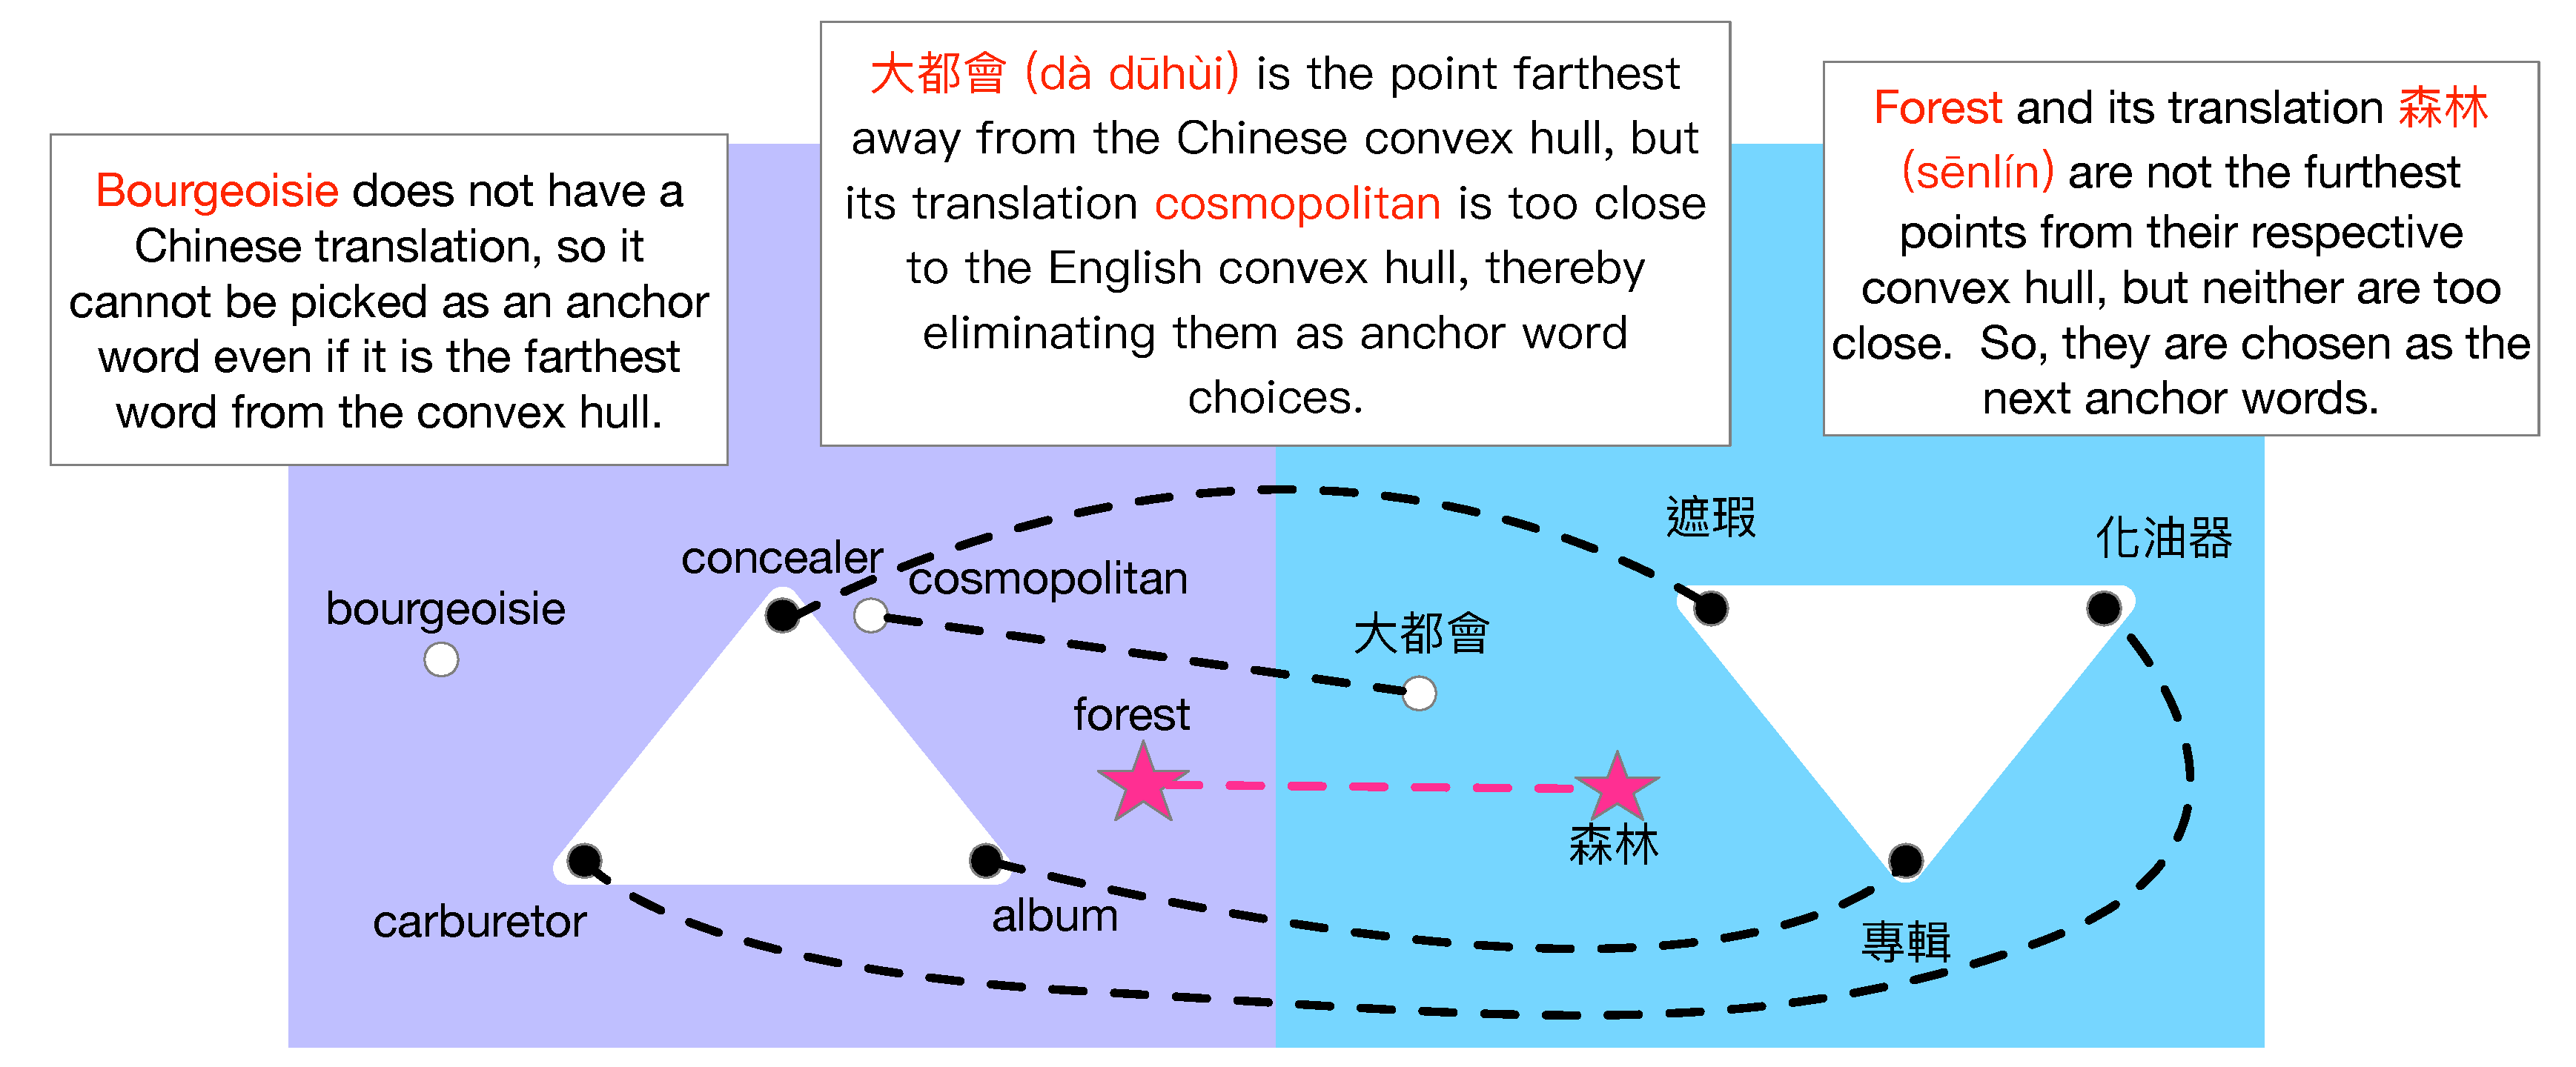
\includegraphics[width=\textwidth]{multi_anchors.pdf}
  \caption{Selecting anchor links for multilingual
    anchoring.  The purple (blue) area represents the conditional
    distribution space of words in the English (Chinese) corpus.  The white triangle designates the space spanned
    by chosen anchor words.  Dashed lines depict anchor links across
    spaces.  Black points denote words already chosen as anchors,
    white points are unchosen words, and pink stars are most optimal anchors for the current iteration.  Multilingual anchors should maximize area spanned by white triangles in both spaces.}
  \label{fig:anchors}
\end{figure}  

\subsection{Multilingual anchoring}
  \label{sec:multilingual}


If there is only one anchor word for each topic, our goal of building a coherent multilingual topic model would fail.  Any imperfection in the dictionary would scupper the topic model.  Fortunately, \etalcite{Arora}{arora-2013} assert that there exist many anchor word choices for a topic.  Even if we reduce the pool for candidate anchors, we can still find suitable anchor words for each topic.  Recall that anchor words are the vertices to the convex hull of words in the conditional distribution space (Section~\ref{sec:background}).  Finding the actual vertices of the convex hulls is too expensive, so FastAnchorWords searches for a set of anchors with maximal span.  This span should approximate the convex hull of~$\bar{Q}$.  Without a large enough span, we can never find accurate approximations for words in the conditional distribution space.  All words~$w$ will have indistinguishable conditional distributions (Figure~\ref{fig:span}).  As a result, every topic will have indistinct word distributions and the resulting topics will be copies of one another.

To maximize span of anchor words, FastAnchorWords~\cite{arora-2013} chooses anchor word~$s_k$ such that
\begin{equation}
  s_k = \argmax_{w} \, d\left(\qspan{ \bar{Q} } {s_1} {s_{k-1}}, \bar{Q}_{w}\right), 
\end{equation}
where~$d(P,i)$ is defined as the Euclidean distance from point~$i$ to subspace~$P$, or the norm of the projection of~$i$ onto the orthogonal complement of~$P$.

To extend the greedy approach to multilingual settings, we need anchor words that can guide topic inference in \emph{multiple} languages.  This motivates our approach for linking words with a dictionary.  By choosing linked anchor words, the algorithm can align topics cross-lingually so that the aligned topics form one multilingual topic.  However, randomly choosing translation pairs as anchor links will not produce coherent multilingual topics.  We need multilingual anchors that also inherit the geometric properties of monolingual anchors.  So, the span of anchor words should be maximized in both languages for optimal topic inference.  To clearly state our objective, we define~$P_j^{(l)}$ as the subspace spanned by~$j$ chosen anchor words in the conditional
distribution space of language~$l$,  
\begin{equation}
  P_j^{(l)} = \qspan{\bar{Q}^{(l)}}{s_1^{(l)} }{s_{j}^{(l)}}.
\end{equation}
Word~$w$ is a good choice of a $k^{th}$ anchor if $\bar{Q}_w$ is far enough from~$P_{k-1}^{(l)}$ so that having $\bar{Q}_w$ as an additional vertex can greatly expand span of anchors. A word might be a great choice for an anchor in one language, but we cannot select it if its translation is a poor choice for the other language (Figure~\ref{fig:anchors}). We need to pick linked words~$w \in \mathcal{L}^{(1)}$ and~$v \in \mathcal{L}^{(2)}$ such
that~$w$ is far from~$P_{k-1}^{(1)}$ and~$v$ is also far away
from~$P_{k-1}^{(2)}$.  Then, adding~$w$ and~$v$ as anchor words can increase total span of anchor word set in both languages.  Using this intuition, we maximize the lower bound on the distance from anchor words to~$P_{k-1}^{(1)}$ and~$P_{k-1}^{(2)}$.  We select anchor words~$w$ and~$v$ such that
  \begin{equation}
    \label{eq:multi_anchors}
    s_k^{(1)}, s_k^{(2)} = 
      \argmax_{w, v} 
      \min \left\{ 
        d\left( P_{k-1}^{(1)}, \bar{Q}^{(1)}_{w}\right), d\left(P_{k-1}^{(2)}, \bar{Q}^{(2)}_{v} \right) 
      \right\} 
      \quad \mbox{ subject to } (w, v) \in \mathcal{B}.
  \end{equation}
We greedily select anchors~$s_k^{(1)} \in \mathcal{L}^{(1)}, s_k^{(2)}
\in \mathcal{L}^{(2)}$ such that Equation~\ref{eq:multi_anchors} is satisfied on every iteration~$k$.  Words with multiple translations
are elegantly addressed: if an anchor word~$w$ is picked already, then
it is not likely to be picked again.  The algorithm expands both convex hulls simultaneously with each iteration. Indeed, more translations aid our anchor search because there will be more linked anchors to choose from.  Even if the algorithm chooses anchor words similar in meaning within the same language, interactivity can help remove duplicate topics (Section~\ref{sec:interface}).  After picking a set of anchor words for each language,
multilingual anchoring follows FastAnchorWords (Section~\ref{sec:anchoring}).  Topic matrices~$A^{(1)}$ and
$A^{(2)}$ are separately recovered (Equations~\ref{eq:anchor},~\ref{eq:topic}).  These matrices are the output of
multilingual anchoring.  In the next sections, we show how
\mtanchor further updates~$A^{(1)}$ and~$A^{(2)}$ based on human feedback.


  \paragraph{Lacking dictionary entries.}
  If dictionary entries are scarce, then we cannot
  constrain the anchor words to only be words from the dictionary.
  So, we independently find anchor words for each language using
  RecoverL2.  This reduction to monolingual settings resembles other cross-lingual models: Joint\abr{lda} reduces to \abr{lda} and
  \abr{ptlda} reduces to \abr{tlda} when there are no dictionary
  entries~\cite{jagarlamudi-2010, hu-2014-ptlda}.

  \paragraph{Predicting labels from topics.}
  \label{sec:predict}
  Multilingual anchoring is an unsupervised method, but the topic distribution acts as a low-dimensional representation for each document~\cite{bengio-2013, xiao-2013, rastogi-2015}.  To infer the topic distribution of documents, we pass in the topic matrices as inputs into variational inference~\citep{blei-2003}, where topic variational parameter~$\beta$ is fixed and only document variational parameter~$\gamma$ is fitted.  Then, we train a linear \abr{svm} on the topic distributions of documents~\citep{fan-2008} to classify document labels.

\begin{figure}
  \centering
  \frame{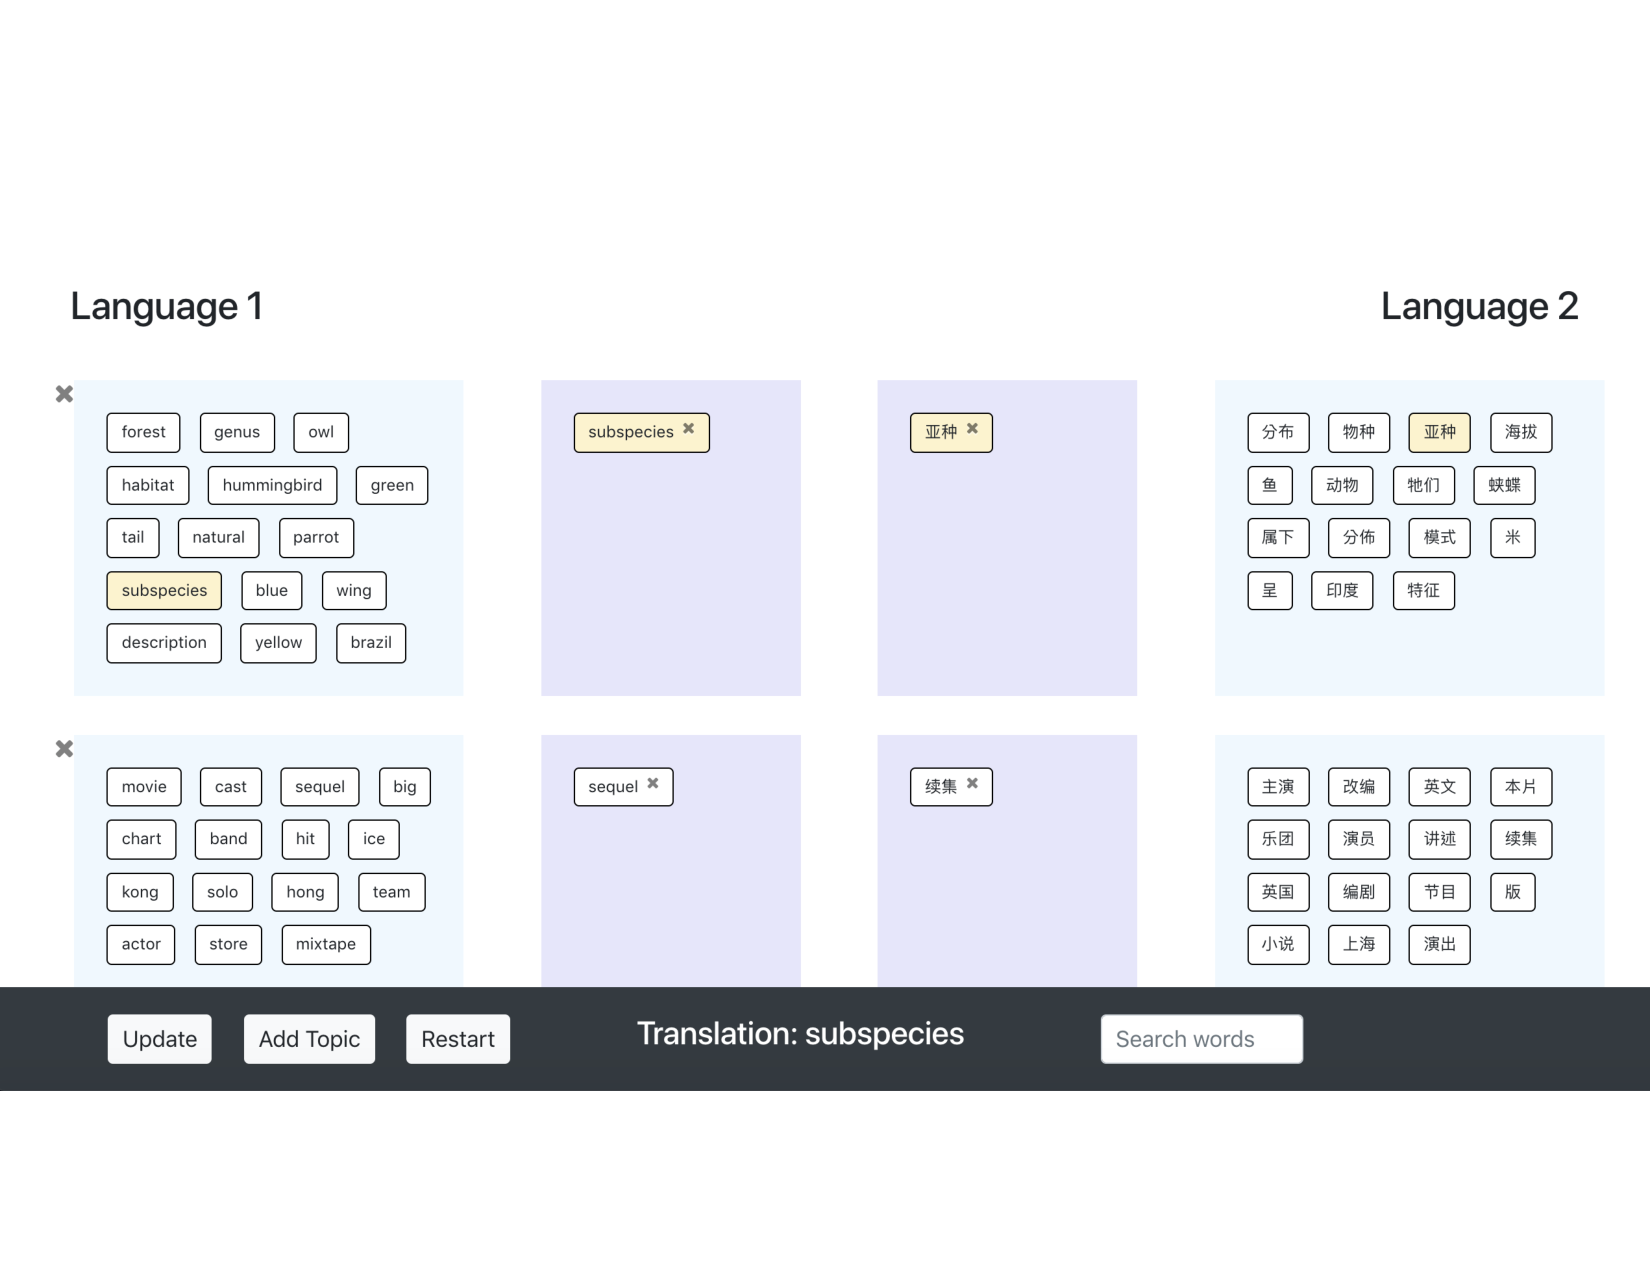
\includegraphics[width=\textwidth]{ui_final.pdf}}
  \caption{The user interface for exploring topics in English and Chinese documents.  Anchor words are in the center, while the most likely words for each topic are on the left and right sides of the interface.  The user can drag words from the side and add them as anchor words.  When the user hovers over ``\zh{亞種}{(y\`azh\v ong)}'', then its translation, ``subspecies'', appears at the bottom of the screen.  When the user presses on the word, all occurrences of it and its translation are highlighted in yellow. Users can type words in the ``Search words'' box to find which words are in the vocabulary.  These features help the user explore topics in an unfamiliar language.}
  \label{fig:ui}
\end{figure}

\subsection{Interactive topic alignment}
\label{sec:interface}

Multilingual anchoring uses translations to find anchor words that
can lead to better topics for both languages.  However, we cannot
completely rely on dictionary entries to construct the topic model.
In reality, translations may not be available, could
be a poor fit for the dataset, or might be wrong.  In
addition to problems with the dictionary, the data may be too noisy,
or the anchoring algorithm returns a topic model unsuited for our
needs (e.g., if a user needs to separate news from opinion and the
topic model puts them together).  Thus, we incorporate interactivity
into \mtanchor so that we can extract linguistic and cultural
knowledge from humans.

First, \mtanchor takes in a comparable corpora and a bilingual dictionary as inputs.  Next, it uses multilingual anchoring
(Section~\ref{sec:multilingual}) to find sets of anchor words for
each language. After the algorithm recovers topic matrices, the
interface shows information about the topic model.  The user can press on the red ``X'' to delete any incoherent or duplicate topics (Figure~\ref{fig:ui}). The user can also add new topics by pressing on ``Add Topics''.  The interface will create a new blank row beneath the existing topics.  Then, the user can add words as anchors to the new topic.  These features are similar to the ones used for interactively modeling monolingual topics~\cite{lund-2017}.


Once the user finishes choosing anchor words for each topic, they press ``Update Topics''.  This is a signal for \mtanchor to retrieve new anchor words from the interface and run multiword anchoring
(Section~\ref{sec:multiword}).  The algorithm approximates~$\bar{Q}_w$ for every word $w$ in the vocabulary and then recomputes the topic matrices for each language.  When \mtanchor finds new topics, the user can see the updated topics on the interface.  At this point, anchors no longer have to be linked by dictionary entries because \mtanchor does not select anchors based on Equation~\ref{eq:multi_anchors}. After the initial alignment, users define anchors and customize the topic model to their own needs.  


